\section{Time Follower's: an overview}
\label{exo:time_follower}

Time Follower's aims at providing an exocentric view of a mobile 
robot using an egocentric-mounted camera. The approach is simple: it is 
based on the use of previously recorded first-person images to provide 
comprehensible third-person imagery. A 3D representation of the robot 
is overlapped to such images in order to get the work done. A graphical
representation of the system is depicted in figure \ref{fig:exocentric}, 
while figure \ref{fig:virtualexocentric} shows an example of what appears 
to the end user.

\begin{figure}[!h]
  \begin{center}
    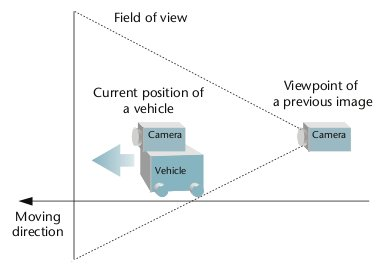
\includegraphics[width=200pt]{img/exocentric_vision.jpg}
    \caption{The \morduc{} robotic platform}
    \label{fig:exocentric}
  \end{center}
\end{figure}

\begin{figure}[!h]
  \begin{center}
    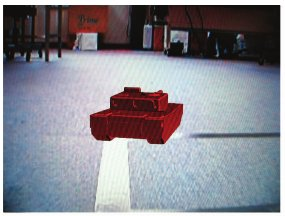
\includegraphics[width=200pt]{img/virtual_exocentric.jpg}  %robot pic
    \caption{A virtual exocentric vision example}
    \label{fig:virtualexocentric}
  \end{center}
\end{figure}

Key issues of such a system are:

\begin{itemize}
\item how to choose the \textit{best} image
\item how to determine the \textit{right} place to draw the robot
\end{itemize}

As for the first issue, the \textit{best} image is the one that allows 
the generation of the \textit{most comprehensible} external robot view.
\cite{sugimoto} provides a set of three effective metrics to 
determine which, of a set of previously recorded images, is the 
one to be chosen.
\\
Once the image is chosen, where to overlap the 3D robot representation 
is quite complex. It is not only a matter of \textit{where} draw the robot
on the image, but also of \textit{how} to set up lighting, robot dimensions,
perspective to make the end user not aware of the fact that what he is
seeing is not the actual environment.
\\
The issues introduced above will be deeply analyzed in the following 
of this document.
